% =============================================================================
%  main.tex
%  -----------------------------------------------------------------------------
%  A LaTeX template for political science manuscripts.
%  English-first, with full Chinese (CJK) support via XeLaTeX + xeCJK.
%  英文为主的学术论文 LaTeX 模板，内置中文支持（XeLaTeX + xeCJK）。
%
%  COMPILE (编译方式):
%     xelatex main.tex
%     bibtex  main        (if you use \cite / \citep / \citet)
%     xelatex main.tex
%     xelatex main.tex
%
%  Folders (目录结构):
%     text/    -- section files (正文分节文件)
%     tables/  -- table files    (表格文件)
%     pics/    -- figure files   (图片文件, PDF)
%     pic-tex/ -- TikZ source of figures (图片的 TikZ 源文件, 单独编译为 PDF)
% =============================================================================

\documentclass[12pt]{article}

% ---- Fonts & CJK support (must be loaded before inputting settings) ----
\usepackage{fontspec}   % XeLaTeX font management
\usepackage{xeCJK}      % Chinese support

% ---- General packages used by the body text ----
\usepackage{graphicx}     % figures
\usepackage{subcaption}   % subfigures
\usepackage{longtable}
\usepackage{array}
\usepackage{makecell}
\usepackage{ragged2e}

% ---- Global preamble settings (fonts, margins, line spacing, tables, math,
%      citations, hyperlinks) ----
% =============================================================================
%  A_PreambleSettings.tex  --  global preamble settings.
%  Central place for fonts, margins, line spacing, tables, math, citations,
%  and hyperlinks. Edit once; affects the whole manuscript.
%  全局导言区设置：字体、页边距、行距、表格、数学、引用与超链接。
% =============================================================================

% -----------------------------------------------------------------------------
%  CJK FONTS  --  pick whatever is installed on your machine.
%  Windows: SimSun / SimHei / FangSong ; macOS: Songti SC / Heiti SC ;
%  Linux: Noto Serif CJK SC / Noto Sans CJK SC.
%  IMPORTANT: set the CJK fonts BEFORE loading newtxtext/newtxmath, otherwise
%  fontspec may report spurious "font cannot be found" errors on Windows TTC
%  fonts. 注意：中文字体设置须在 newtx 字体之前，否则 Windows 下可能误报。
% -----------------------------------------------------------------------------
\IfFontExistsTF{SimSun}{%
  \setCJKmainfont[AutoFakeBold=2.5]{SimSun}%   % fake bold for Chinese bold text
  \setCJKsansfont{SimHei}%
  \setCJKmonofont{FangSong}%
}{%
  \IfFontExistsTF{Noto Serif CJK SC}{%
    \setCJKmainfont[AutoFakeBold=2.5]{Noto Serif CJK SC}%
    \setCJKsansfont{Noto Sans CJK SC}%
    \setCJKmonofont{Noto Sans Mono CJK SC}%
  }{%
    % Fallback: xeCJK will use the default CJK font (may produce warnings).
  }%
}

% -----------------------------------------------------------------------------
%  MATH  --  amsmath/amssymb/amsthm must ALL be loaded BEFORE newtxmath
%  (newtxmath loads amsmath internally and redefines \Bbbk / \openbox).
%  注意：amsmath、amssymb、amsthm 必须全部先于 newtxmath 加载。
% -----------------------------------------------------------------------------
\usepackage[tbtags]{amsmath}
\usepackage{amssymb}
\usepackage{amsthm,verbatim}

% -----------------------------------------------------------------------------
%  FONTS  --  Times-like text and math fonts (load AFTER CJK fonts and the
%  AMS packages)
% -----------------------------------------------------------------------------
\usepackage{newtxtext,newtxmath}   % Times New Roman style text & math

% newtxtext sets \defaultfontfeatures{Extension=.otf, ...}, which would leak
% into xeCJK's deferred (lazy) CJK font loads and cause spurious fontspec
% errors. Reset it immediately. 复位默认字体特性，避免影响 xeCJK 的中文字体。
\defaultfontfeatures{}

% -----------------------------------------------------------------------------
%  PAGE GEOMETRY & LINE SPACING
% -----------------------------------------------------------------------------
\RequirePackage[
  left=1in,
  right=1in,
  top=1in,
  bottom=1in,
  headheight=0pt,
  headsep=0pt]{geometry}

\setlength{\headsep}{5pt}      % distance between header and body
\linespread{1.35}              % 1.35x line spacing

% -----------------------------------------------------------------------------
%  LISTS
% -----------------------------------------------------------------------------
\RequirePackage[shortlabels,inline]{enumitem} % custom lists with inline labels
\setlist{nolistsep}            % compact lists

% -----------------------------------------------------------------------------
%  FIGURES
% -----------------------------------------------------------------------------
\usepackage{graphicx}
\graphicspath{{pics/}{pic-tex/}}   % default search paths for images
\usepackage{subcaption}
\captionsetup[subfigure]{width=0.8\textwidth}
\usepackage{tikz}                  % TikZ for vector graphics
\usetikzlibrary{calc}

% -----------------------------------------------------------------------------
%  TABLES
% -----------------------------------------------------------------------------
\usepackage{booktabs}              % publication-quality rules
\usepackage{threeparttable}        % tables with notes
\usepackage{adjustbox}             % resize wide tables (max width=\textwidth)
\usepackage{longtable}             % tables spanning multiple pages
\usepackage{makecell}              % multi-line cells

% -----------------------------------------------------------------------------
%  CAPTIONS
% -----------------------------------------------------------------------------
\RequirePackage[font=small,labelfont={bf}]{caption}
\captionsetup{justification=centering}
\captionsetup[table]{skip=3pt}
\captionsetup[figure]{skip=3pt}

% -----------------------------------------------------------------------------
%  THEOREMS
% -----------------------------------------------------------------------------
\newtheorem{theorem}{Theorem}
\newtheorem{lemma}{Lemma}
\newtheorem{proposition}{Proposition}
\newtheorem{corollary}{Corollary}
\newtheorem{assumption}{Assumption}
\newtheorem{hypothesis}{Hypothesis}

% -----------------------------------------------------------------------------
%  MATH OPERATORS
% -----------------------------------------------------------------------------
\DeclareMathOperator*{\argmin}{arg\,min}
\DeclareMathOperator*{\argmax}{arg\,max}
\DeclareMathOperator*{\plim}{plim}

% -----------------------------------------------------------------------------
%  CITATIONS & BIBLIOGRAPHY
% -----------------------------------------------------------------------------
\usepackage[round,sort&compress]{natbib}
\setlength{\bibsep}{2.5pt}
\def\bibfont{\footnotesize}

% -----------------------------------------------------------------------------
%  MISC  --  pdfpages, setspace, landscape, floats
% -----------------------------------------------------------------------------
% NOTE: paragraph indentation is set to 2em in main.tex (standard for
% Chinese manuscripts). If you prefer no indentation with vertical spacing
% between paragraphs, uncomment the parskip package below and remove the
% \setlength{\parindent}{2em} line in main.tex.
% 注意：main.tex 中将段首缩进设为 2em（中文习惯）。若希望段落间空行、
% 无缩进，可取消下行注释并在 main.tex 中删除缩进设置。
% \usepackage{parskip}
\usepackage{pdfpages}   % include PDF pages as-is
\usepackage{setspace}   % line spacing adjustments
\usepackage{pdflscape}  % landscape pages
\usepackage{afterpage}  % typeset content after current page
\usepackage{float}      % [H] placement
\renewcommand{\abstractname}{Abstract}

% -----------------------------------------------------------------------------
%  HYPERLINKS  --  load last
% -----------------------------------------------------------------------------
\usepackage{hyperref}
\RequirePackage{xcolor}
\definecolor{winered}{rgb}{0.5,0,0}   % dark red link color
\hypersetup{colorlinks,linkcolor={winered},citecolor={winered},urlcolor={winered}}
\usepackage{url}


% ---- Paragraph indentation: 2em (standard for Chinese manuscripts) ----
\setlength{\parindent}{2em}

% =============================================================================
%  TITLE PAGE  --  REPLACE with your own title and author information.
%  请替换为你自己的论文标题与作者信息。
% =============================================================================
\title{\textbf{Your Manuscript Title:\\ A Reproducible LaTeX Template for Political Science}}

\author{
  Your Name\thanks{Department, University. Email: your.name@university.edu}
  \and
  Co-author Name\thanks{Corresponding author. Department, University. Email: coauthor@university.edu}
}

\date{\today}

\begin{document}

\maketitle

% =============================================================================
%  ABSTRACT  --  bilingual example. Keep the English version as the main text;
%  the Chinese version below is optional and can be removed for English-only
%  submissions. 摘要示例：英文为主，中文可选。
% =============================================================================
\begin{abstract}
% =============================================================================
%  text/abstract.tex
%  Bilingual abstract example: English first (main text), Chinese optional.
%  摘要示例：英文为主（正文），中文为可选翻译。
% =============================================================================

\textbf{Abstract.} This is a template for political science manuscripts.
Replace this paragraph with your own abstract. The template supports English
text with optional Chinese text, author--year citations (\texttt{\textbackslash citep},
\texttt{\textbackslash citet}), equations, publication-quality tables, and
TikZ figures. It compiles with XeLaTeX and BibTeX; no additional configuration
is required beyond installing a TeX distribution and a CJK font.

% 中文摘要（可选，英文投稿时可删除）
\textbf{摘要.} 这是一个政治学论文 LaTeX 模板。请将本段替换为你自己的摘要。
本模板支持英文为主、中文为辅的排版（XeLaTeX + xeCJK），内置 author--year
引用格式（natbib）、公式、三线表与 TikZ 图形。

\medskip
\textbf{Keywords:} political science; LaTeX template; bilingual typesetting;
XeLaTeX; reproducible research
% 关键词（可选）：政治学；LaTeX 模板；双语排版；XeLaTeX；可复现研究

\end{abstract}

\newpage

% =============================================================================
%  MAIN TEXT  --  structure mirrors a typical political science manuscript.
%  Each section is split into per-section files under text/.
%  正文结构：与常见政治学论文一致，各节拆分为 text/ 下的独立文件。
% =============================================================================

\section{INTRODUCTION}
% =============================================================================
%  text/introduction.tex
%  Introduction: demonstrates citations, Chinese paragraph, and a bulleted
%  list of contributions. Replace all content with your own.
%  引言示例：演示引用、中英混排段落与要点列表。
% =============================================================================

A growing literature examines how political elites shape state capacity and
political survival \citep{author2018book,author2020example}. Scholars have
shown that cohesive elite networks can both strengthen the state and threaten
the ruler, a tension sometimes called the ruler's dilemma
\citep[e.g.,][]{author2019chapter}. This paper develops a dynamic framework
that explains how rulers' strategic choices shift across different political
conditions.

% 中文段落示例：中英文段落交错排布（英文为主、中文为辅）。
% 中文段落示例：中英文段落交错排布（英文为主、中文为辅）。
当统治者的权力稳固时，培养具有凝聚力的精英网络有助于提升国家能力；
当权力脆弱时，统治者则可能转而分化精英联盟以阻止挑战。
本文的理论框架将这两种策略统一在一个基于边际收益的决策模型之中，
并说明理性的统治者总是选择边际收益最大的策略。

This paper makes three contributions. First, it provides a unified framework
that connects elite management with state-building outcomes. Second, it
introduces a novel empirical strategy for measuring elite network structure.
Third, it applies the framework to a salient historical case with rich
temporal variation in the ruler's power security.

Our empirical analysis proceeds as follows. Section~\ref{sec:elite-ruler}
presents the theoretical argument. Section~\ref{sec:case-background}
introduces the historical background of the case. Section~\ref{sec:sample}
describes the research design, and Section~\ref{sec:main-results} reports the
results. Section~\ref{sec:conclusion} concludes.

% 贡献列表示例（如需编号列表，请将 itemize 改为 enumerate）
Our main findings can be summarized as follows:
\begin{itemize}
  \item Well-connected elites enjoy better promotion prospects when the
        ruler's authority is consolidated.
  \item The same elites become targets of suppression when the ruler's
        authority is challenged.
  \item These dynamics have lasting consequences for state capacity.
\end{itemize}


\section{THE ARGUMENT}
% =============================================================================
%  text/THE ARGUMENT/intro.tex
%  Roadmap for the theory section. Replace with your own text.
%  理论部分导读。
% =============================================================================

This section develops the theoretical framework.
Section~\ref{sec:elite-ruler} discusses the interaction between elites and
rulers and its implications for state capacity.
Section~\ref{sec:ruler-dilemma} introduces a dynamic, marginal-returns-based
model of the ruler's dilemma.
Section~\ref{sec:four-strategies} classifies four archetypical strategies
that rulers adopt under different combinations of authority stability and
policy priorities.

% 本节提出理论框架：2.1 讨论精英与统治者的互动；2.2 提出基于边际收益的
% 统治者二难困境动态模型；2.3 归纳统治者在不同权力稳定程度与政策优先
% 组合下采取的四类典型策略。


\subsection{Elite--Ruler Relations and State Capacity}
\label{sec:elite-ruler}
% =============================================================================
%  text/THE ARGUMENT/elite-ruler-relations.tex
%  Theory subsection: demonstrates theorem / hypothesis environments and
%  citations. Replace with your own argument.
%  理论小节示例：演示定理与假设环境。
% =============================================================================

We begin with a simple observation. Elites capable of coordinating collective
action are essential for state-building: they staff bureaucracies, implement
policies, and solve collective-action problems that fragment societies
\citep{author2020example,author2018book}. Yet the same capacity for collective
action that makes elites valuable also makes them dangerous. An elite network
powerful enough to defend the state can, under the right conditions, threaten
the ruler who heads it.

\begin{assumption}[Elite capacity is double-edged]
Elite networks that contribute to state capacity can also be mobilized to
challenge the ruler.
\end{assumption}

Building on this premise, we characterize the ruler's problem as one of
allocating scarce attention and resources between two competing goals:
consolidating personal power and investing in state capacity.

\begin{proposition}[Security determines elite management]
When the ruler's authority is insecure, the marginal returns to power
consolidation exceed the marginal returns to state-building, and the ruler
responds by fragmenting elite networks. When the ruler's authority is
secure, the ranking is reversed, and the ruler fosters elite cohesion.
\end{proposition}

\begin{hypothesis}[Promotion]
Officials who occupy central positions in elite networks enjoy better
promotion prospects when the ruler's authority is consolidated.
\label{hyp:promotion}
\end{hypothesis}

\begin{hypothesis}[Suppression]
Officials who occupy central positions in elite networks are more likely to
be suppressed when the ruler's authority is challenged.
\label{hyp:suppression}
\end{hypothesis}

% 中文对照（可选）
% 命题与假设的中文翻译可放在此处，或删除。
Hypotheses~\ref{hyp:promotion} and~\ref{hyp:suppression} are tested
empirically in Section~\ref{sec:main-results}.


\subsection{The Dynamic Logic of the Ruler's Dilemma}
\label{sec:ruler-dilemma}
% =============================================================================
%  text/THE ARGUMENT/ruler-dilemma.tex
%  Theory subsection: demonstrates an equation and marginal-returns logic.
%  理论小节示例：演示公式排版。
% =============================================================================

We formalize the ruler's decision as a comparison of marginal returns.
Let $R$ denote the ruler's probability of political survival and $S$ denote
the level of state capacity. The ruler allocates a fixed budget $B$ between
two activities: power consolidation $p$ and state-building $s$, with
$p+s=B$. The ruler solves

\begin{equation}
\max_{p,s} \; U(R(p),\, S(s)) \quad \text{subject to} \quad p+s=B,
\label{eq:ruler-problem}
\end{equation}

where $U$ is strictly increasing in both arguments.

The key comparative statics follow from the curvature of $R(\cdot)$.
When authority is insecure, $R$ is steep: each additional unit of
consolidation substantially reduces the probability of being overthrown, so
$\partial R/\partial p \gg \partial S/\partial s$ and the optimum shifts
toward fragmentation of elite networks. When authority is secure, $R$ is
flat, $\partial S/\partial s$ dominates, and the ruler invests in cohesive
elite networks instead.

\begin{equation}
\text{Strategy}^* =
\begin{cases}
\text{fragment elites}, & \text{if } \dfrac{\partial R}{\partial p}
  > \dfrac{\partial S}{\partial s};\\[2ex]
\text{foster elite cohesion}, & \text{if } \dfrac{\partial S}{\partial s}
  \geq \dfrac{\partial R}{\partial p}.
\end{cases}
\label{eq:strategy-choice}
\end{equation}

% 中文对照（可选）
% 式 (1) 刻画统治者在权力巩固与政权建设之间的资源配置问题；
% 式 (2) 给出边际收益比较下的最优策略选择。
This simple framework, summarized in equations~\eqref{eq:ruler-problem} and
\eqref{eq:strategy-choice}, generates the four strategies discussed in
Section~\ref{sec:four-strategies}.


\subsection{A Fourfold Strategy Framework}
\label{sec:four-strategies}
% =============================================================================
%  text/THE ARGUMENT/fourfold-strategy.tex
%  Theory subsection: demonstrates a 2x2 typology table with booktabs.
%  理论小节示例：演示 2x2 分类表格（三线表）。
% =============================================================================

Combining the ruler's authority security (secure vs.\ fragile) with the
priority given to state-building (high vs.\ low) yields a fourfold typology of
ruling strategies, summarized in Table~\ref{tab:fourfold}.

% 表 1：四类典型策略的 2x2 分类（booktabs 三线表示例）
\begin{table}[htbp]
  \centering
  \caption{A Fourfold Typology of Ruling Strategies}
  \label{tab:fourfold}
  \begin{tabular}{p{3.2cm} p{4.6cm} p{4.6cm}}
    \toprule
    & \textbf{State-building priority: high} & \textbf{State-building priority: low} \\
    \midrule
    \textbf{Authority secure}    & Foster elite cohesion;
                                   invest in institutions. &
                                   Consolidate personal networks;
                                   status quo politics. \\
    \addlinespace
    \textbf{Authority fragile}   & Co-opt elites; share rents to
                                   buy survival. &
                                   Fragment elite coalitions;
                                   purge potential challengers. \\
    \bottomrule
  \end{tabular}
  \begin{tablenotes}
    \footnotesize
    \item \textit{Note:} This table is a placeholder demonstrating the
    \texttt{booktabs} + \texttt{threeparttable} table format. Replace the
    content with your own typology.
  \end{tablenotes}
\end{table}

We expect the empirical case to display a transition across these cells over
time, as the ruler's authority security varies (Section~\ref{sec:ruler-power-dynamics}).


\section{HISTORICAL BACKGROUND}
% =============================================================================
%  text/HISTORICAL BACKGROUND/intro.tex
%  Roadmap for the background section (placeholder).
%  背景部分导读（占位）。
% =============================================================================

This section is a placeholder for the background part of your paper.
Section~\ref{sec:background} demonstrates narrative paragraphs with
citations, and Section~\ref{sec:developments} demonstrates how to include a
figure. Replace the files \texttt{background.tex} and
\texttt{developments.tex} with your own content.

% 本节为论文背景部分的占位。两个小节分别演示叙述段落与插图；
% 请以你自己的内容替换 background.tex 与 developments.tex。


\subsection{The Case and Its Background}
\label{sec:case-background}
% =============================================================================
%  text/HISTORICAL BACKGROUND/case-background.tex
%  Case background: demonstrates narrative paragraphs and a \citet citation.
%  案例背景示例。
% =============================================================================

% 请将此节替换为你自己的案例背景叙述。
Newly established regimes typically coalesce under leaders backed by cohorts
of capable elites. A robust literature establishes that elite capacity for
collective action is central to state-building \citep{author2018book,author2020example}.
Extensive evidence from developing regions, for instance, demonstrates that
elite fragmentation impairs rulers' ability to project authority and retards
the development of fiscal systems and public administration.

% 中文段落示例（可选）
% 新兴政体通常在由能干精英群体支持的领导者领导下凝聚起来。大量研究证实，
% 精英阶层的集体行动能力对于国家建设至关重要；精英在地理或派系线上的
% 碎片化会削弱统治者推行权威的能力，并阻碍财政体系与行政机构的发展。

Yet rulers' rational calculations do not invariably favor elite cohesion.
As \citet{author2019chapter} argues, the strategic imperatives of political
survival may diverge sharply from the requirements of national prosperity.
History bears this out: many prominent rulers fell not to external adversaries
or mass uprisings, but to challenges orchestrated by their closest associates.

% 历史背景部分的其余内容（事件梳理、关键时间线等）请在此展开。
Herein lies the fundamental tension this paper studies: an elite network
powerful enough to sustain the state simultaneously poses a latent threat to
the ruler's own position. The case examined below offers sharp temporal
variation in the ruler's power security, enabling us to observe how the same
ruler adopted diametrically opposed strategies under different conditions.

Chinese-language scholarship makes closely related arguments about the
relationship between institutional change and state capacity
\citep{zhang2018example}; engaging this literature is encouraged when
relevant to your case.


\subsection{Ruler Power Dynamics over Time}
\label{sec:ruler-power-dynamics}
% =============================================================================
%  text/HISTORICAL BACKGROUND/ruler-power-dynamics.tex
%  Documents temporal variation in ruler power security; references a figure.
%  统治者权力动态示例：引用图片。
% =============================================================================

We organize the case narrative around three periods that differ in the
security of the ruler's authority. In the first period, the ruler commanded
unrivalled prestige following the founding of the regime, and authority over
both party and state was consolidated. In the second period, policy failures
eroded the ruler's standing, and senior elites mounted increasingly open
challenges to his leadership. In the third period, the ruler reasserted
authority through large-scale reshuffles of the elite.

% 中文对照（可选）
% 本文围绕统治者权力稳固程度不同的三个阶段组织案例叙述：建国初期权力
% 巩固；政策失败后权威受损、精英公开挑战；随后统治者通过大规模人事调整
% 重新确立权威。

Figure~\ref{fig:timeline} provides a stylized illustration of the
power-security dynamics across these periods. The figure is generated from a
standalone TikZ source file (\texttt{pic-tex/example-tikz/example-tikz.tex})
and included as a compiled PDF, following the project's figure workflow.

% 图 1：示意时间线（TikZ 独立编译后插入）
\begin{figure}[htbp]
  \centering
  
\includegraphics[width=0.85\textwidth]{example-figure.pdf}
  \caption{Stylized Timeline of Ruler Power Security Across Three Periods}
  \label{fig:timeline}
\end{figure}

This temporal variation provides the identification strategy exploited in the
research design (Section~\ref{sec:sample}): the same ruler, confronting the
same elite network, adopted different strategies under different conditions of
power security.


\section{RESEARCH DESIGN}
% =============================================================================
%  text/RESEARCH DESIGN/intro.tex
%  Roadmap for the research design section (placeholder).
%  研究设计部分导读（占位）。
% =============================================================================

This section is a placeholder for the research design part of your paper.
Section~\ref{sec:sample} introduces the data and sample,
Section~\ref{sec:key-variable} defines the key variable, and
Sections~\ref{sec:outcome-1} and~\ref{sec:outcome-2} define the outcomes.
Replace the corresponding files under \texttt{text/RESEARCH DESIGN/} with
your own content.

% 本节为论文研究设计部分的占位：样本、关键变量与结果变量。
% 请替换 text/RESEARCH DESIGN/ 目录下的对应文件。


\subsection{Sample}
\label{sec:sample}
% =============================================================================
%  text/RESEARCH DESIGN/sample.tex
%  Demonstrates a descriptive-statistics table. Content is placeholder.
%  演示描述统计表；内容为占位，请替换。
% =============================================================================

This subsection demonstrates how to present descriptive statistics. Put your
table files in \texttt{tables/} and \texttt{\textbackslash input} them here
or from \texttt{text/APPENDIX/tables.tex}. The table below uses generic
variable names and placeholder numbers.

% 中文对照（可选）
% 本小节演示描述统计表的排版方式：表格文件放在 tables/ 目录，
% 在此处或 text/APPENDIX/tables.tex 中引用。下表使用通用变量名与占位数字。
Table~\ref{tab:descriptive} reports descriptive statistics for the main
variables used in the analysis.

% =============================================================================
%  tables/table-descriptive.tex
%  Example descriptive statistics table (generic variable names and
%  placeholder numbers). 描述统计示例表（通用变量名与占位数字）。
% =============================================================================

\begin{table}[htbp]
  \centering
  \caption{Descriptive Statistics (Placeholder Values)}
  \label{tab:descriptive}
  \begin{threeparttable}
  \small
  \begin{tabular}{lccccc}
    \toprule
    Variable & N & Mean & SD & Min & Max \\
    \midrule
    Variable A & 1,502 & 0.042 & 0.061 & 0.000 & 0.412 \\
    Variable B & 1,502 & 2.556 & 1.730 & 1.000 & 7.000 \\
    Variable C & 1,502 & 2.270 & 1.542 & 1.000 & 6.000 \\
    Variable D & 1,502 & 1929.8 & 8.4 & 1911 & 1949 \\
    \bottomrule
  \end{tabular}
  \begin{tablenotes}
    \footnotesize
    \item \textit{Note:} PLACEHOLDER values. Replace with your own
    descriptive statistics.
  \end{tablenotes}
  \end{threeparttable}
\end{table}



\subsection{Key Explanatory Variable}
\label{sec:key-variable}
% =============================================================================
%  text/RESEARCH DESIGN/key-variable.tex
%  Demonstrates a definition-style equation. Content is placeholder.
%  演示定义式公式排版；内容为占位，请替换。
% =============================================================================

This subsection demonstrates how to define a key variable with a display
equation. For a generic illustration, consider a quantity defined as a sum
over a set of indices:

\begin{equation}
K(i) \;=\; \sum_{j \in J(i)} w_{ij} \, x_j .
\label{eq:example-3}
\end{equation}

% 中文对照（可选）
% 式 (3) 是一个通用的指标定义示例。请将本小节替换为你自己的变量定义。
Intuitively, $K(i)$ aggregates the weighted values $x_j$ over the index set
$J(i)$ with weights $w_{ij}$. This is only a placeholder definition; replace
it with the definition of your own key variable, and mention the data or
materials used to construct it.


\subsection{Outcome 1: Promotion and State-Building}
\label{sec:outcome-promotion}
% =============================================================================
%  text/RESEARCH DESIGN/outcome-promotion.tex
%  Outcome 1: promotion and state-building. Demonstrates an equation.
%  结果变量一：晋升与国家建设。
% =============================================================================

Our first outcome measures career advancement and contributions to
state-building. Career advancement is coded from official position records
using a standard rank scale. State-building is measured by the elite's
appointments to positions responsible for constructing state institutions
(fiscal administration, public services, and bureaucratic agencies), weighted
by the importance of each post.

% 中文对照（可选）
% 第一个结果变量衡量职务晋升与国家建设贡献：晋升依据官方职位记录编码；
% 国家建设贡献以精英在财政、公共服务与行政机构等关键职位上的任职衡量。

We estimate the following specification using OLS:

\begin{equation}
Promotion_i = \alpha + \beta \, Centrality_i + \mu_j + \mathbf{X}_i'
\boldsymbol{\gamma} + \varepsilon_i ,
\label{eq:promotion}
\end{equation}

where $Promotion_i$ is the outcome for elite $i$, $Centrality_i$ is the
network centrality measure defined in equation~\eqref{eq:betweenness},
$\mu_j$ are fixed effects for the elite's origin province $j$, $\mathbf{X}_i$
is a vector of controls (year of entry into politics, organizational
experience, and education), and standard errors are clustered at the province
level.


\subsection{Outcome 2: Challenge and Purge}
\label{sec:outcome-purge}
% =============================================================================
%  text/RESEARCH DESIGN/outcome-purge.tex
%  Outcome 2: challenge and purge. Demonstrates an equation.
%  结果变量二：挑战与清洗。
% =============================================================================

Our second outcome measures the elite's challenge to the ruler and the
severity of subsequent suppression. Challenge is coded from records of
criticism of the ruler's policies in internal meetings and publications.
Suppression is coded from official records of removal from office, demotion,
and other punitive measures, using a severity scale.

% 中文对照（可选）
% 第二个结果变量衡量精英对统治者的挑战程度与随后遭受清洗的严重程度。

We estimate the following specification:

\begin{equation}
Purge_i = \alpha + \beta \, Centrality_i + \mu_j + \mathbf{X}_i'
\boldsymbol{\gamma} + \varepsilon_i ,
\label{eq:purge}
\end{equation}

where all variables are defined as in equation~\eqref{eq:promotion}.
Testing Hypothesis~\ref{hyp:suppression} amounts to examining whether
$\beta>0$ in equation~\eqref{eq:purge} during the period in which the ruler's
authority was challenged.


\section{RESULTS}
% =============================================================================
%  text/RESULTS/intro.tex
%  Roadmap for the results section (placeholder).
%  结果部分导读（占位）。
% =============================================================================

This section is a placeholder for the results part of your paper.
Section~\ref{sec:main-results} demonstrates how to present main estimates
with a regression table and a figure, and Section~\ref{sec:robustness}
demonstrates subfigures. Replace the files under
\texttt{text/RESULTS/} with your own content.

% 本节为论文结果部分的占位：主要结果与稳健性检验。
% 请替换 text/RESULTS/ 目录下的对应文件。


\subsection{Main Results}
\label{sec:main-results}
% =============================================================================
%  text/RESULTS/main-results.tex
%  Main results: demonstrates a regression-table input and figure reference.
%  主要结果示例：引用回归表与图片。
% =============================================================================

Table~\ref{tab:main-promotion} reports estimates of
equation~\eqref{eq:promotion} for the period in which the ruler's authority
was consolidated. Consistent with Hypothesis~\ref{hyp:promotion}, the
coefficient on network centrality is positive and statistically significant
across specifications, including the full set of controls.

\begin{figure}[htbp]
  \centering
  
\includegraphics[width=0.8\textwidth]{example-figure.pdf}
  \caption{Marginal Effects of Network Centrality on Promotion (Placeholder)}
  \label{fig:marginal-effects}
\end{figure}

% 中文对照（可选）
% 表 B1 报告权力巩固时期晋升方程的估计结果：网络中心性的系数为正且显著，
% 与假设 1 一致。图 2 展示了核心变量对晋升的边际效应（示意图，请替换）。
Figure~\ref{fig:marginal-effects} visualizes the marginal effects.

Table~\ref{tab:main-purge} reports estimates of equation~\eqref{eq:purge}
for the period in which the ruler's authority was challenged. Consistent with
Hypothesis~\ref{hyp:suppression}, the coefficient on network centrality is
positive and statistically significant: precisely the elites who were
rewarded during the consolidation period became targets of suppression when
the ruler's authority wavered.

% 表 B2 报告权力受挑战时期清洗方程的估计结果：网络中心性系数为正且显著，
% 与假设 2 一致——权力巩固时期受奖赏的精英在权威动摇时反而成为清洗对象。
These two sets of results jointly support the dynamic framework developed in
Section~\ref{sec:elite-ruler}.


\subsection{Robustness Checks}
\label{sec:robustness}
% =============================================================================
%  text/RESULTS/robustness.tex
%  Demonstrates a subfigure environment. Content is placeholder.
%  演示子图环境；内容为占位，请替换。
% =============================================================================

This subsection demonstrates how to place two figures side by side with the
\texttt{subcaption} package. Replace the placeholder figures and the text
with your own robustness checks.

% 中文对照（可选）
% 本小节演示用 subcaption 宏包并排摆放两张子图（图 3a、图 3b）。
% 请替换为你的稳健性检验结果。
\begin{figure}[htbp]
  \centering
  \begin{subfigure}[b]{0.48\textwidth}
    \centering
    
\includegraphics[width=\textwidth]{example-figure/example-figure.pdf}
    \caption{First specification}
    \label{fig:sub-a}
  \end{subfigure}
  \hfill
  \begin{subfigure}[b]{0.48\textwidth}
    \centering
    
\includegraphics[width=\textwidth]{example-figure/example-figure.pdf}
    \caption{Second specification}
    \label{fig:sub-b}
  \end{subfigure}
  \caption{Subfigure Example (Placeholder)}
  \label{fig:robustness}
\end{figure}

Figures~\ref{fig:sub-a} and~\ref{fig:sub-b} illustrate the intended layout.


\section{CONCLUSION}
\label{sec:conclusion}
% =============================================================================
%  text/conclusion.tex
%  Conclusion example. Replace with your own concluding remarks.
%  结论示例：请替换为你自己的结论。
% =============================================================================

This paper has developed and tested a dynamic framework of ruler--elite
relations. When power is secure, rulers cultivate cohesive elite networks to
advance state capacity; when power is fragile, they fragment elite coalitions
to forestall challenges. The empirical results are consistent with these
theoretical expectations and survive a battery of robustness checks reported
in the Appendix.

% 中文结论（可选）
本文构建并检验了一个关于统治者—精英关系的动态分析框架：权力稳固时，
统治者培养凝聚性的精英网络以推进国家建设；权力脆弱时，统治者则分化
精英联盟以防范挑战。实证结果与理论预期一致，并在一系列稳健性检验中
保持稳健（见附录）。

Our findings carry implications beyond the specific case. They suggest that
the long-term developmental trajectory of newly established regimes depends
critically on the security of the ruler's authority in the early years of
consolidation. Future research could extend the framework to other regions
and time periods, and explore the micro-mechanisms through which elite
networks shape policy outcomes \citep{author2024working}.


\newpage

% =============================================================================
%  REFERENCES  --  aeaown.bst is a Harvard (author-year) style.
% =============================================================================
\bibliographystyle{aeaown}
\bibliography{references}

\newpage

% =============================================================================
%  APPENDIX  --  table and figure numbering restarts with B/A prefixes.
% =============================================================================
\appendix

\section*{APPENDIX}
\addcontentsline{toc}{section}{APPENDIX}

\section{Tables}
\label{app:tables}
\setcounter{table}{0}
\renewcommand{\thetable}{B\arabic{table}}
% =============================================================================
%  text/APPENDIX/tables.tex
%  Appendix tables. Input your table files from tables/ here.
%  附录表格：在此引入 tables/ 目录下的表格文件。
% =============================================================================

\input{tables/table-main-1}

\input{tables/table-main-2}


\section{Figures}
\label{app:figures}
\setcounter{figure}{0}
\renewcommand{\thefigure}{A\arabic{figure}}
% =============================================================================
%  text/APPENDIX/figures.tex
%  Appendix figures. Two workflows are demonstrated:
%    1) A compiled PDF placed in pics/ and included with \includegraphics.
%    2) A standalone TikZ source in pic-tex/ compiled separately to PDF.
%  附录图片：演示两种图片工作流（预编译 PDF 与 TikZ 独立编译）。
% =============================================================================

% ---- Workflow 1: pre-compiled PDF in pics/ ----
\begin{figure}[htbp]
  \centering
  
\includegraphics[width=0.9\textwidth]{example-figure.pdf}
  \caption{Marginal Benefit Dynamics (Placeholder Figure)}
  \label{fig:appendix-figure-1}
\end{figure}

% ---- Workflow 2: TikZ source compiled to PDF in pic-tex/ ----
% =============================================================================
%  pic-tex/example-tikz/example-tikz.tex
%  FIGURE WRAPPER: includes the pre-compiled PDF (example-tikz-source.pdf)
%  produced from example-tikz-source.tex in the same folder. Input this file
%  from text/APPENDIX/figures.tex or any other place.
%  图片包装文件：插入同目录下由 example-tikz-source.tex 编译得到的 PDF。
% =============================================================================

\begin{figure}[htbp]
  \centering
  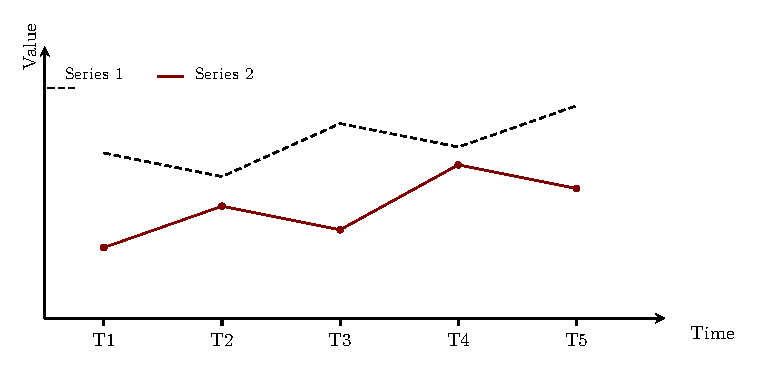
\includegraphics[width=0.8\textwidth]{pic-tex/example-tikz/example-tikz-source.pdf}
  \vspace{0.5em}
  \caption{A Generic Example Figure (Placeholder)}
  \label{fig:appendix-tikz}
  \vspace{0.5em}
  \caption*{\footnotesize \justifying \textit{Note:} This is a placeholder
  figure demonstrating the TikZ workflow. Compile
  \texttt{pic-tex/example-tikz/example-tikz-source.tex} to regenerate the
  PDF, then replace the drawing with your own content.}
\end{figure}



\end{document}
